\documentclass[conference]{IEEEtran}
\IEEEoverridecommandlockouts

% -----------------------------------------------------------------------------
% PACKAGE IMPORTS
% -----------------------------------------------------------------------------
\usepackage{amsmath,amssymb,amsfonts}
\usepackage{algorithmic}
\usepackage{graphicx}
\usepackage{textcomp}
\usepackage{xcolor}
\usepackage{booktabs}
\usepackage{tabularx}
\usepackage{multirow}
\usepackage{listings}
\usepackage{url}
\usepackage{cite}
\usepackage{microtype}
\usepackage{tikz}
\usetikzlibrary{shapes.geometric, arrows, positioning, fit, backgrounds, calc}

\usepackage[hidelinks]{hyperref}

% -----------------------------------------------------------------------------
% LISTINGS CONFIGURATION
% -----------------------------------------------------------------------------
\lstset{
    basicstyle=\ttfamily\scriptsize,
    breaklines=true,
    frame=single,
    captionpos=b,
    tabsize=2,
    keepspaces=true,
    showstringspaces=false
}

% -----------------------------------------------------------------------------
% METADATA AND TITLE
% -----------------------------------------------------------------------------
\title{SpamAdapt: A Comparative Study of Full Fine-Tuning, Low-Rank Adaptation, and Weight-Decomposed Low-Rank Adaptation for SMS Spam Detection}

\author{
    \IEEEauthorblockN{Akash\IEEEauthorrefmark{1}}
    \IEEEauthorblockA{\IEEEauthorrefmark{1}Department of Computer Science and Engineering\\
    [Institution / University Name Placeholder], [City, Country Placeholder]\\
    Email: [author.email@institution.edu Placeholder]}
}

\begin{document}

\maketitle

% -----------------------------------------------------------------------------
% ABSTRACT
% -----------------------------------------------------------------------------
\begin{abstract}
Short Message Service (SMS) spam poses severe financial, psychological, and security risks, including phishing, fraud, and credential harvesting. Although pretrained bidirectional transformer encoders, such as BERT, have established state-of-the-art predictive performance in text classification, conventional Full Fine-Tuning requires updating and persisting all 109.5 million parameters for each task. This presents severe storage, computational, and edge-deployment bottlenecks. In this work, we propose and empirically evaluate \textbf{SpamAdapt}, a systematic machine learning and software engineering framework comparing Full Fine-Tuning against two parameter-efficient adaptation paradigms: Low-Rank Adaptation (LoRA) and Weight-Decomposed Low-Rank Adaptation (DoRA), applied to \texttt{google-bert/bert-base-uncased} for SMS spam detection. Using the benchmark UCI SMS Spam Collection ($N=5,160$ cleaned unique messages) with a stratified 70\%/15\%/15\% split ($N_{\text{test}}=774$), we demonstrate that LoRA ($r=8, \alpha=16$) achieves a Test Accuracy of 98.32\% and a Macro $F_1$ of 96.12\%, retaining 99.7\% of the Full Fine-Tuning baseline Macro $F_1$ (96.40\%) while training only 296,450 parameters (a 369.3$\times$ parameter reduction) and reducing serialized weight storage from 417.67~MB to 1.14~MB (a 366.4$\times$ disk saving). DoRA achieves 98.19\% accuracy and 95.84\% Macro $F_1$ while yielding a lower test cross-entropy loss (0.0779 vs. 0.0783 for LoRA), but incurs an inference latency overhead (110.00~ms vs. 92.05~ms on CPU) due to runtime directional normalization. Remarkably, all three adaptation methods exhibit invariant spam recall (91.75\%, detecting 89 of 97 spam messages). Finally, we engineer an interactive, privacy-preserving Streamlit web application featuring real-time PyTorch inference, dynamic model switching, in-memory caching, and automated verification suites.
\end{abstract}

% -----------------------------------------------------------------------------
% KEYWORDS
% -----------------------------------------------------------------------------
\begin{IEEEkeywords}
SMS spam detection, BERT, transformer encoder, Full Fine-Tuning, LoRA, DoRA, PEFT, text classification, model efficiency, natural language processing.
\end{IEEEkeywords}

% -----------------------------------------------------------------------------
% SECTION I: INTRODUCTION
% -----------------------------------------------------------------------------
\section{Introduction}
\label{sec:intro}

The proliferation of mobile telecommunications has rendered Short Message Service (SMS) an indispensable communication medium for personal, commercial, and financial authentication transactions. However, this ubiquity has simultaneously established SMS as an attractive attack vector for malicious actors. Unsolicited text messages, commonly termed SMS spam, have evolved far beyond benign marketing annoyances into sophisticated smishing (SMS phishing), financial fraud, malware distribution, and identity theft operations~\cite{almeida2011sms}. 

Automated spam classification faces unique linguistic hurdles compared to email filtering: SMS messages are severely constrained in character length, frequently incorporate non-standard abbreviations, phonetic spellings, and creative evasion orthography, and exhibit substantial class imbalance~\cite{almeida2011sms}. Historically, feature engineering coupled with traditional machine learning models (e.g., Naive Bayes, Support Vector Machines, and Random Forests) provided acceptable baseline filtering but struggled with out-of-vocabulary tokens and syntactic ambiguity.

The advent of the Transformer architecture~\cite{vaswani2017attention} and pretrained contextualized representations, notably the Bidirectional Encoder Representations from Transformers (BERT)~\cite{devlin2019bert}, fundamentally transformed Natural Language Processing (NLP). BERT's bidirectional self-attention mechanisms capture intricate semantic, structural, and contextual dependencies across tokens. Consequently, fine-tuning BERT on downstream sequence classification tasks routinely yields superior performance.

Despite these advantages, standard Full Fine-Tuning updates all underlying model parameters ($109.5\times 10^6$ parameters for BERT-base). Storing and serving independent checkpoints of over 400~MB for each application or task variation introduces severe operational challenges, particularly in memory-constrained edge gateways, mobile client environments, and multi-tenant cloud microservices.

To mitigate this computational and storage footprint, Parameter-Efficient Fine-Tuning (PEFT) techniques have gained immense traction. Low-Rank Adaptation (LoRA)~\cite{hu2022lora} freezes the pretrained backbone weights and introduces trainable rank decomposition matrices into the multi-head self-attention projections. More recently, Weight-Decomposed Low-Rank Adaptation (DoRA)~\cite{liu2024dora} was proposed to bridge the subtle performance gap between LoRA and Full Fine-Tuning by decomposing weight matrices into magnitude and directional components, applying LoRA solely to the directional update.

In this paper, we present \textbf{SpamAdapt}, a comprehensive empirical research study and production-grade software framework that systematically evaluates Full Fine-Tuning, LoRA, and DoRA under identical, reproducible experimental conditions for SMS spam detection.

% -----------------------------------------------------------------------------
% SECTION II: PROBLEM STATEMENT & RESEARCH OBJECTIVES
% -----------------------------------------------------------------------------
\section{Problem Formulation and Objectives}
\label{sec:problem_objectives}

\subsection{Problem Statement}
Let $\mathcal{X}$ denote the space of SMS text messages, and let $\mathcal{Y} = \{0, 1\}$ represent the ground-truth binary label space, where $0$ denotes legitimate communication (\textit{ham}) and $1$ denotes fraudulent or unsolicited communication (\textit{spam}). Given a pretrained bidirectional transformer encoder $\mathcal{M}_{\Theta_0}$ parameterized by $\Theta_0 \in \mathbb{R}^D$, downstream adaptation produces a task-specific classifier $\mathcal{M}_{\Theta^*}$. 

The core research question is: \textit{Can parameter-efficient adaptation methods (LoRA and DoRA), which update only a minute fraction of model parameters ($\Delta \Theta \ll \Theta_0$), achieve classification performance statistically and practically parity-equivalent to Full Fine-Tuning on SMS spam detection, while substantially reducing training time, serialized storage requirements, and inference latency?}

\subsection{Research Objectives}
To address this question rigorously, the project defines six measurable objectives:
\begin{enumerate}
    \item \textbf{Data Pipeline Engineering}: Ingest, clean, and deduplicate the raw UCI SMS Spam Collection, establishing a deterministic, stratified 70\%/15\%/15\% split protected by cryptographic SHA-256 validation.
    \item \textbf{Model Adaptation Implementation}: Formulate and implement Full Fine-Tuning, LoRA, and DoRA on \texttt{google-bert/bert-base-uncased} with rigorous parameter isolation.
    \item \textbf{Empirical Evaluation}: Evaluate all three adaptation regimes on the identical held-out test split ($N=774$) across Accuracy, Precision, Recall, $F_1$, and Macro $F_1$.
    \item \textbf{Efficiency Benchmarking}: Measure trainable parameter counts, serialized adapter/checkpoint sizes, process memory deltas (RSS), per-message inference latency profiles (mean, median, P95), and throughput.
    \item \textbf{Interactive Demonstration}: Build an interactive, multi-tab Streamlit web application providing live SMS prediction, cached model loading, transparent metrics display, and privacy-preserving ephemeral session history.
    \item \textbf{Scientific Rigor & Reproducibility}: Perform exhaustive validation to guarantee metric consistency across JSON artifacts, confusion matrices, and live test executions.
\end{enumerate}

% -----------------------------------------------------------------------------
% SECTION III: RESEARCH QUESTIONS & CONTRIBUTIONS
% -----------------------------------------------------------------------------
\section{Research Questions and Contributions}
\label{sec:rq_contrib}

\subsection{Research Questions}
We formulate four specific research questions (RQs):
\begin{itemize}
    \item \textbf{RQ1}: What is the trade-off in predictive performance (Macro $F_1$, Spam Precision, and Spam Recall) when switching from Full Fine-Tuning to parameter-efficient LoRA and DoRA?
    \item \textbf{RQ2}: Does weight-decomposition in DoRA improve predictive performance over standard LoRA on short-text sequence classification?
    \item \textbf{RQ3}: How do LoRA and DoRA compare in terms of disk storage, memory footprint, and CPU inference latency relative to Full Fine-Tuning?
    \item \textbf{RQ4}: Can an adapter-based NLP pipeline be integrated seamlessly into a responsive, privacy-compliant web interface without external API dependencies?
\end{itemize}

\subsection{Key Contributions}
The key contributions of this paper are summarized as follows:
\begin{itemize}
    \item \textbf{Reproducible Benchmarking Framework}: We deliver an end-to-end, modular NLP research codebase ([`src/`](file:///c:/Users/Akash/Documents/Scam_Detection/SpamAdapt/src)) supporting automated data loading, deterministic stratified splitting, tokenization, training, evaluation, and benchmarking.
    \item \textbf{Rigorous PEFT Analysis}: We present an empirical comparison showing that LoRA retains 99.7\% of Full Fine-Tuning Macro $F_1$ with a 369.3$\times$ parameter reduction and 366.4$\times$ storage reduction.
    \item \textbf{DoRA Behavior Characterization}: We document that while DoRA yields a lower test cross-entropy loss, its runtime column-wise normalization introduces an inference latency penalty on CPU compared to LoRA.
    \item \textbf{Production-Ready Interactive System}: We develop a polished Streamlit web application ([`app/main.py`](file:///c:/Users/Akash/Documents/Scam_Detection/SpamAdapt/app/main.py)) featuring real-time inference, dynamic hardware detection, in-memory model caching, and strict data privacy compliance.
\end{itemize}

% -----------------------------------------------------------------------------
% SECTION IV: BACKGROUND & RELATED WORK
% -----------------------------------------------------------------------------
\section{Background and Related Work}
\label{sec:background}

\subsection{Transformer Encoders and BERT}
The Transformer architecture~\cite{vaswani2017attention} eliminated recurrent dependencies by relying entirely on multi-head self-attention. BERT (\textit{Bidirectional Encoder Representations from Transformers})~\cite{devlin2019bert} instantiated a multi-layer bidirectional transformer encoder trained on massive unlabeled corpora using Masked Language Modeling (MLM) and Next Sentence Prediction (NSP). For sequence classification, BERT prefixes every tokenized input with a special classification token, \texttt{[CLS]}. The final hidden state corresponding to \texttt{[CLS]} serves as an aggregate sequence representation, which is fed to a task-specific linear projection layer.

Crucially, BERT is an encoder model designed for representation extraction and sequence labeling; it is fundamentally distinct from autoregressive generative large language models (such as GPT).

\subsection{Parameter-Efficient Fine-Tuning (PEFT)}
As pretrained language models expanded in capacity, Full Fine-Tuning—updating all parameters $\Theta_0$ via backpropagation—became computationally and logistically prohibitive. Early PEFT alternatives introduced serial or parallel adapter layers within the transformer blocks. However, these adapter layers frequently introduced inference latency overheads due to sequential computation bottlenecks.

\subsection{Low-Rank Adaptation (LoRA)}
To address adapter latency, Hu et al.~\cite{hu2022lora} introduced LoRA. Drawing upon prior findings that parameter updates during adaptation have a low ``intrinsic dimension'', LoRA freezes the pretrained weights $W_0 \in \mathbb{R}^{d \times k}$ and models the weight update $\Delta W$ via low-rank decomposition:
\begin{equation}
\Delta W = \frac{\alpha}{r} B A
\end{equation}
where $B \in \mathbb{R}^{d \times r}$ and $A \in \mathbb{R}^{r \times k}$, with rank $r \ll \min(d, k)$, and $\alpha$ is a constant scaling hyperparameter. Because $W = W_0 + \Delta W$ is linear, the adapter weights can be folded back into $W_0$ at deployment, incurring zero added inference latency.

\subsection{Weight-Decomposed Low-Rank Adaptation (DoRA)}
Liu et al.~\cite{liu2024dora} observed that Full Fine-Tuning exhibits distinct learning dynamics compared to LoRA: Full Fine-Tuning induces complex, non-correlated changes in both the magnitude and directional components of weight matrices, whereas LoRA exhibits a high degree of proportional correlation between magnitude and directional updates. To bridge this dynamic disparity, DoRA decomposes the weight matrix into a trainable magnitude vector $m$ and a directional matrix $V$, applying LoRA updates exclusively to the directional component.

% -----------------------------------------------------------------------------
% SECTION V: DATASET & DATA PREPARATION
% -----------------------------------------------------------------------------
\section{Dataset and Data Preparation}
\label{sec:dataset}

\subsection{Data Source and Preprocessing}
The empirical investigation utilizes the renowned UCI SMS Spam Collection~\cite{almeida2011sms}, loaded programmatically via Hugging Face Datasets (\texttt{ucirvine/sms\_spam}). The raw repository contains 5,574 text entries.

To prevent artificial metric inflation and data leakage, we execute a rigorous, signal-preserving cleaning pipeline via [`src/preprocessing.py`](file:///c:/Users/Akash/Documents/Scam_Detection/SpamAdapt/src/preprocessing.py):
\begin{enumerate}
    \item \textbf{HTML Entity Decoding}: Unescaping HTML entities (e.g., \texttt{\&amp;} $\rightarrow$ \texttt{\&}, \texttt{\&lt;} $\rightarrow$ \texttt{<}).
    \item \textbf{Whitespace Normalization}: Replacing non-standard Unicode spaces (\texttt{\textbackslash u00a0}, \texttt{\textbackslash u200b}) with standard spaces and collapsing redundant spaces.
    \item \textbf{Signal Preservation}: Explicitly retaining uppercase text, punctuation (e.g., ``\texttt{!!!}'', ``\texttt{???}''), phone numbers, currency symbols (\texttt{\$}, \texttt{\pounds}), and URLs, as these tokens constitute vital heuristic markers of spam intent.
    \item \textbf{Deduplication}: Identifying and removing exact message duplicates. In the raw dataset, 414 duplicate records were detected and purged.
\end{enumerate}

Following deduplication, the cleaned corpus comprises exactly 5,160 unique records.

\subsection{Dataset Statistics and Class Imbalance}
Table~\ref{tab:dataset_stats} outlines the structural characteristics of the cleaned dataset. The corpus displays an extreme class imbalance of 7.04:1 (87.56\% ham vs. 12.44\% spam). Legitimate messages average 70.34 characters (14.23 words), whereas spam messages are substantially longer, averaging 137.41 characters (23.70 words), reflecting verbose promotional and phishing phrasing.

\begin{table}[htbp]
\caption{Dataset Summary and Text Characteristics}
\label{tab:dataset_stats}
\centering
\begin{tabular}{lrrr}
\toprule
\textbf{Metric / Attribute} & \textbf{Ham (0)} & \textbf{Spam (1)} & \textbf{Overall} \\
\midrule
Sample Count & 4,518 & 642 & 5,160 \\
Class Percentage & 87.56\% & 12.44\% & 100.0\% \\
Imbalance Ratio & --- & --- & 7.04 : 1 \\
Mean Character Length & 70.34 & 137.41 & 78.68 \\
Median Character Length & 52.00 & 148.00 & 60.00 \\
Mean Word Count & 14.23 & 23.70 & 15.41 \\
Median Word Count & 11.00 & 25.00 & 12.00 \\
Max Character Length & 910 & 224 & 910 \\
\bottomrule
\end{tabular}
\end{table}

\subsection{Stratified Splitting and Integrity Verification}
To guarantee rigorous evaluation without label distribution skew, the corpus is divided into 70\% training ($N=3,612$), 15\% validation ($N=774$), and 15\% test ($N=774$) splits using stratified sampling with a fixed random seed ($\text{seed}=42$).

Table~\ref{tab:splits} reports the exact counts and class distributions across all three partitions. Each split was serialized to disk and locked via cryptographic SHA-256 hashes recorded in [`split_metadata.json`](file:///c:/Users/Akash/Documents/Scam_Detection/SpamAdapt/data/processed/split_metadata.json).

\begin{table}[htbp]
\caption{Stratified Partition Distribution ($seed=42$)}
\label{tab:splits}
\centering
\begin{tabular}{lrrrr}
\toprule
\textbf{Partition} & \textbf{Ham (0)} & \textbf{Spam (1)} & \textbf{Total} & \textbf{Spam \%} \\
\midrule
Train (70\%) & 3,163 & 449 & 3,612 & 12.43\% \\
Validation (15\%) & 678 & 96 & 774 & 12.40\% \\
Test (15\%) & 677 & 97 & 774 & 12.53\% \\
\midrule
\textbf{Total} & \textbf{4,518} & \textbf{642} & \textbf{5,160} & \textbf{12.44\%} \\
\bottomrule
\end{tabular}
\end{table}

% -----------------------------------------------------------------------------
% SECTION VI: SYSTEM ARCHITECTURE
% -----------------------------------------------------------------------------
\section{System Architecture}
\label{sec:system_arch}

The SpamAdapt framework is organized into two primary operational pipelines: an \textbf{Offline Research Pipeline} and an \textbf{Online Inference Pipeline}. Figure~\ref{fig:sys_arch} illustrates the holistic system architecture.

\begin{figure*}[htbp]
\centering
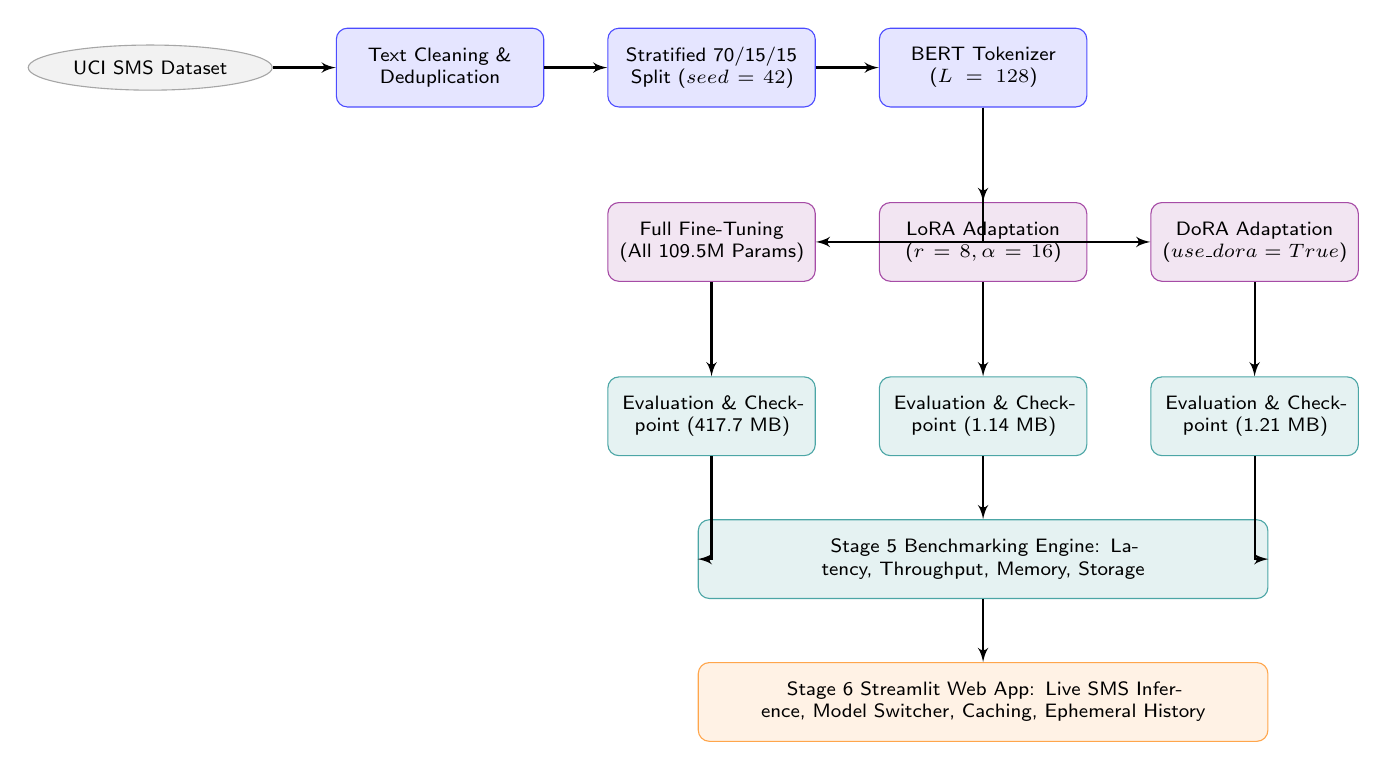
\begin{tikzpicture}[
    node distance=1.2cm and 1.0cm,
    block/.style={rectangle, draw=blue!70, fill=blue!10, rounded corners, text width=2.4cm, text centered, minimum height=1.0cm, font=\scriptsize\sffamily},
    modelblock/.style={rectangle, draw=violet!70, fill=violet!10, rounded corners, text width=2.4cm, text centered, minimum height=1.0cm, font=\scriptsize\sffamily},
    evalblock/.style={rectangle, draw=teal!70, fill=teal!10, rounded corners, text width=2.4cm, text centered, minimum height=1.0cm, font=\scriptsize\sffamily},
    uiblock/.style={rectangle, draw=orange!70, fill=orange!10, rounded corners, text width=2.4cm, text centered, minimum height=1.0cm, font=\scriptsize\sffamily},
    cloudblock/.style={ellipse, draw=gray!70, fill=gray!10, text centered, font=\scriptsize\sffamily},
    line/.style={draw, -latex', thick}
]

% Data Ingestion
\node [cloudblock] (rawdata) {UCI SMS Dataset};
\node [block, right=0.8cm of rawdata] (cleaning) {Text Cleaning \& Deduplication};
\node [block, right=0.8cm of cleaning] (splitting) {Stratified 70/15/15 Split ($seed=42$)};
\node [block, right=0.8cm of splitting] (tokenizer) {BERT Tokenizer ($L=128$)};

% Models
\node [modelblock, below=1.2cm of tokenizer] (lora) {LoRA Adaptation ($r=8, \alpha=16$)};
\node [modelblock, left=0.8cm of lora] (fullft) {Full Fine-Tuning (All 109.5M Params)};
\node [modelblock, right=0.8cm of lora] (dora) {DoRA Adaptation ($use\_dora=True$)};

% Evaluation
\node [evalblock, below=1.2cm of fullft] (eval_ft) {Evaluation \& Checkpoint (417.7 MB)};
\node [evalblock, below=1.2cm of lora] (eval_lora) {Evaluation \& Checkpoint (1.14 MB)};
\node [evalblock, below=1.2cm of dora] (eval_dora) {Evaluation \& Checkpoint (1.21 MB)};

% Benchmarking & Web App
\node [evalblock, below=0.8cm of eval_lora, text width=7.0cm] (benchmark) {Stage 5 Benchmarking Engine: Latency, Throughput, Memory, Storage};
\node [uiblock, below=0.8cm of benchmark, text width=7.0cm] (webapp) {Stage 6 Streamlit Web App: Live SMS Inference, Model Switcher, Caching, Ephemeral History};

% Connectors
\path [line] (rawdata) -- (cleaning);
\path [line] (cleaning) -- (splitting);
\path [line] (splitting) -- (tokenizer);

\path [line] (tokenizer) |- (fullft);
\path [line] (tokenizer) -- (lora);
\path [line] (tokenizer) |- (dora);

\path [line] (fullft) -- (eval_ft);
\path [line] (lora) -- (eval_lora);
\path [line] (dora) -- (eval_dora);

\path [line] (eval_ft) |- (benchmark);
\path [line] (eval_lora) -- (benchmark);
\path [line] (eval_dora) |- (benchmark);

\path [line] (benchmark) -- (webapp);

\end{tikzpicture}
\caption{SpamAdapt System Architecture: Data preprocessing, parallel fine-tuning tracks, evaluation, efficiency benchmarking, and live interactive Streamlit deployment.}
\label{fig:sys_arch}
\end{figure*}

\begin{itemize}
    \item \textbf{Offline Pipeline}: Consists of automated raw dataset retrieval, minimal text cleaning, stratified splitting, BERT tokenization, model training (Full FT, LoRA, and DoRA), held-out evaluation, and computational benchmarking. Checkpoint weights and metrics are archived under [`experiments/`](file:///c:/Users/Akash/Documents/Scam_Detection/SpamAdapt/experiments) and [`results/`](file:///c:/Users/Akash/Documents/Scam_Detection/SpamAdapt/results).
    \item \textbf{Online Pipeline}: The Streamlit web application loads the cached base model and selected adapter dynamically, tokenizes user input or curated samples on the fly, computes softmax classification probabilities, and displays real-time latency and safety indicators.
\end{itemize}

% -----------------------------------------------------------------------------
% SECTION VII: MATHEMATICAL FOUNDATIONS
% -----------------------------------------------------------------------------
\section{Mathematical Foundations}
\label{sec:math}

\subsection{BERT Sequence Representation and Self-Attention}
Let an input SMS sequence be tokenized into a sequence of $L$ tokens $X = (x_1, x_2, \dots, x_L)$, where $x_1 = \texttt{[CLS]}$ and $L \le 128$. Each token is mapped to an initial embedding vector $e_i \in \mathbb{R}^{d_{\text{model}}}$, where $d_{\text{model}} = 768$.

Within each of the 12 transformer layers, multi-head self-attention computes query ($Q$), key ($K$), and value ($V$) projections:
\begin{equation}
Q = X W_Q, \quad K = X W_K, \quad V = X W_V
\end{equation}
where $W_Q, W_K, W_V \in \mathbb{R}^{d_{\text{model}} \times d_k}$, with $d_k = d_{\text{model}} / h = 64$ across $h = 12$ attention heads. Scaled dot-product attention is defined as:
\begin{equation}
\text{Attention}(Q, K, V) = \text{softmax}\left(\frac{Q K^T}{\sqrt{d_k}}\right) V
\end{equation}
The final representation corresponding to the classification token is denoted as $h_{\text{[CLS]}} \in \mathbb{R}^{d_{\text{model}}}$.

\subsection{Sequence Classification Head}
For binary classification, a linear projection head with parameters $W_c \in \mathbb{R}^{2 \times d_{\text{model}}}$ and bias $b_c \in \mathbb{R}^2$ computes raw classification logits $z \in \mathbb{R}^2$:
\begin{equation}
z = W_c h_{\text{[CLS]}} + b_c = [z_0, z_1]^T
\end{equation}
Class probabilities are derived via the softmax activation function:
\begin{equation}
P(y = c \mid X) = \frac{e^{z_c}}{e^{z_0} + e^{z_1}}, \quad c \in \{0, 1\}
\end{equation}
The binary cross-entropy loss over a training batch of size $B$ is:
\begin{equation}
\mathcal{L} = -\frac{1}{B} \sum_{i=1}^B \left[ y_i \log P(y_i = 1 \mid X_i) + (1 - y_i) \log P(y_i = 0 \mid X_i) \right]
\end{equation}

\subsection{Full Fine-Tuning Formulation}
In Full Fine-Tuning, all parameters $\Theta = \{\Theta_{\text{backbone}}, W_c, b_c\}$ are unfrozen. Gradient updates are applied via AdamW:
\begin{equation}
\Theta^{(t+1)} = \Theta^{(t)} - \eta \cdot \frac{\hat{m}_t}{\sqrt{\hat{v}_t} + \epsilon} - \eta \lambda \Theta^{(t)}
\end{equation}
where $\eta = 2\times 10^{-5}$ is the learning rate, $\lambda = 0.01$ is the weight decay, and $\hat{m}_t, \hat{v}_t$ are bias-corrected first and second moment estimates. Total trainable parameters equal $|\Theta| = 109,483,778$.

\subsection{LoRA Formulation}
In LoRA~\cite{hu2022lora}, the base transformer weights $W_0 \in \mathbb{R}^{d \times k}$ are frozen ($\nabla_{W_0} \mathcal{L} = 0$). Trainable rank decomposition matrices $A \in \mathbb{R}^{r \times k}$ and $B \in \mathbb{R}^{d \times r}$ are injected into the attention projections:
\begin{equation}
W = W_0 + \Delta W = W_0 + \frac{\alpha}{r} B A
\end{equation}
where $r = 8$ is the rank and $\alpha = 16$ is the scaling factor. In SpamAdapt, LoRA adapters are injected into the \texttt{query} and \texttt{value} projection layers across all 12 transformer blocks, alongside the trainable classification head ($W_c, b_c$).

\subsection{DoRA Formulation}
DoRA~\cite{liu2024dora} decomposes a weight matrix into its magnitude vector $m \in \mathbb{R}^{1 \times k}$ and directional matrix $V \in \mathbb{R}^{d \times k}$:
\begin{equation}
W = m \odot \frac{V}{\|V\|_c}
\end{equation}
where $\odot$ denotes element-wise broadcasting multiplication, and $\|\cdot\|_c$ denotes the column-wise $L_2$ norm:
\begin{equation}
\|V\|_{c, j} = \sqrt{\sum_{i=1}^d V_{ij}^2}, \quad j \in \{1, \dots, k\}
\end{equation}
Setting $V = W_0 + \Delta W$ where $\Delta W = \frac{\alpha}{r} B A$, the decomposed weight representation becomes:
\begin{equation}
W = m \odot \frac{W_0 + \frac{\alpha}{r} B A}{\left\| W_0 + \frac{\alpha}{r} B A \right\|_c}
\end{equation}
At initialization, $m = \|W_0\|_c$ and $B = 0$, ensuring that $W = W_0$ exactly at the start of training. During backpropagation, gradients update $m$, $B$, $A$, and the classification head, while $W_0$ remains strictly frozen.

% -----------------------------------------------------------------------------
% SECTION VIII: MODEL IMPLEMENTATION & CONFIGURATION
% -----------------------------------------------------------------------------
\section{Model Implementation and Configuration}
\label{sec:model_config}

All models are instantiated using the Hugging Face Transformers~\cite{wolf2020transformers} and PEFT~\cite{peft2022} libraries built upon PyTorch~\cite{paszke2019pytorch}. Table~\ref{tab:hyperparams} summarizes the exact experimental hyperparameter configurations across all three regimes.

\begin{table}[htbp]
\caption{Experimental Hyperparameter Configuration}
\label{tab:hyperparams}
\centering
\begin{tabular}{lccc}
\toprule
\textbf{Hyperparameter} & \textbf{Full Fine-Tuning} & \textbf{LoRA (PEFT)} & \textbf{DoRA (PEFT)} \\
\midrule
Base Model & \multicolumn{3}{c}{\texttt{google-bert/bert-base-uncased}} \\
Hidden Size ($d_{\text{model}}$) & \multicolumn{3}{c}{768} \\
Transformer Layers & \multicolumn{3}{c}{12} \\
Attention Heads & \multicolumn{3}{c}{12} \\
Max Sequence Length & \multicolumn{3}{c}{128} \\
Number of Epochs & \multicolumn{3}{c}{1} \\
Per-Device Batch Size & \multicolumn{3}{c}{2} \\
Gradient Accumulation Steps & \multicolumn{3}{c}{4} \\
Effective Batch Size & \multicolumn{3}{c}{8} \\
Optimization Steps & \multicolumn{3}{c}{452} \\
Optimizer & \multicolumn{3}{c}{AdamW ($\beta_1=0.9, \beta_2=0.999, \epsilon=10^{-8}$)} \\
Weight Decay & \multicolumn{3}{c}{0.01} \\
Learning Rate & $2\times 10^{-5}$ & $2\times 10^{-4}$ & $2\times 10^{-4}$ \\
Adapter Rank ($r$) & --- & 8 & 8 \\
Adapter Alpha ($\alpha$) & --- & 16 & 16 \\
Adapter Dropout & --- & 0.1 & 0.1 \\
Target Modules & --- & \texttt{query}, \texttt{value} & \texttt{query}, \texttt{value} \\
DoRA Magnitude Mode & --- & False & True \\
\bottomrule
\end{tabular}
\end{table}

\subsection{Parameter Breakdown and Isolation}
Table~\ref{tab:param_breakdown} details the parameter counts verified from [`full_finetuning.json`](file:///c:/Users/Akash/Documents/Scam_Detection/SpamAdapt/results/metrics/full_finetuning.json), [`lora.json`](file:///c:/Users/Akash/Documents/Scam_Detection/SpamAdapt/results/metrics/lora.json), and [`dora.json`](file:///c:/Users/Akash/Documents/Scam_Detection/SpamAdapt/results/metrics/dora.json).

\begin{table}[htbp]
\caption{Parameter Count and Efficiency Comparison}
\label{tab:param_breakdown}
\centering
\begin{tabular}{lrrr}
\toprule
\textbf{Parameter Category} & \textbf{Full Fine-Tuning} & \textbf{LoRA} & \textbf{DoRA} \\
\midrule
Base Backbone & 109,482,240 & 109,482,240 & 109,482,240 \\
Classification Head & 1,538 & 1,538 & 1,538 \\
LoRA $A$ \& $B$ Matrices & 0 & 294,912 & 294,912 \\
DoRA Magnitude Vectors ($m$) & 0 & 0 & 18,432 \\
\midrule
\textbf{Total Parameters} & \textbf{109,483,778} & \textbf{109,780,228} & \textbf{109,798,660} \\
\textbf{Trainable Parameters} & \textbf{109,483,778} & \textbf{296,450} & \textbf{314,882} \\
\textbf{Frozen Parameters} & \textbf{0} & \textbf{109,483,778} & \textbf{109,483,778} \\
\textbf{Trainable Percentage} & \textbf{100.00\%} & \textbf{0.27\%} & \textbf{0.29\%} \\
\textbf{Parameter Reduction} & \textbf{1.0$\times$} & \textbf{369.3$\times$} & \textbf{347.7$\times$} \\
\bottomrule
\end{tabular}
\end{table}

The classification head contributes 1,538 parameters ($768 \times 2$ weights + 2 biases). LoRA introduces 294,912 adapter parameters across 12 layers ($12 \times 2 \times [768 \times 8 + 8 \times 768]$). DoRA introduces an additional 18,432 learnable magnitude parameters ($12 \text{ layers} \times 2 \text{ modules} \times 768 \text{ dimensions}$).

% -----------------------------------------------------------------------------
% SECTION IX: SOFTWARE ARCHITECTURE & PROJECT FILES
% -----------------------------------------------------------------------------
\section{Software Architecture and File Inventory}
\label{sec:software_arch}

\subsection{Physical Codebase Structure}
The complete SpamAdapt repository structure is documented in Listing~\ref{lst:tree}.

\begin{lstlisting}[caption={Verified Directory Structure of the SpamAdapt Project}, label={lst:tree}]
SpamAdapt/
|-- data/
|   |-- raw/raw_sms_spam.csv
|   `-- processed/
|       |-- train.csv (3,612 rows)
|       |-- val.csv (774 rows)
|       |-- test.csv (774 rows)
|       `-- split_metadata.json (SHA-256)
|-- src/
|   |-- config.py
|   |-- data_loader.py
|   |-- preprocessing.py
|   |-- tokenization.py
|   |-- model.py
|   |-- train.py
|   |-- evaluate.py
|   |-- benchmark.py
|   `-- utils.py
|-- experiments/
|   |-- full_finetuning/ (run.py, model/)
|   |-- lora/ (run.py, model/)
|   |-- dora/ (run.py, model/)
|   `-- run_benchmark.py
|-- results/
|   |-- metrics/ (full_finetuning, lora, dora, efficiency_benchmark.json)
|   |-- plots/ (*.png)
|   `-- reports/dataset_summary.json
|-- app/
|   |-- main.py
|   |-- inference.py
|   |-- metrics_loader.py
|   `-- styles.py
|-- test_app.py
|-- verify_stage7.py
|-- requirements.txt
`-- README.md
\end{lstlisting}

\subsection{Module Inventory and Dependencies}
Table~\ref{tab:file_inventory} specifies the core source files, their dependencies, functional responsibilities, and consumer modules.

\begin{table*}[htbp]
\caption{Comprehensive Source File Inventory and Module Connections}
\label{tab:file_inventory}
\centering
\scriptsize
\begin{tabularx}{\textwidth}{l p{3.2cm} p{5.5cm} p{4.0cm}}
\toprule
\textbf{Source File} & \textbf{Direct Dependencies} & \textbf{Main Responsibility} & \textbf{Primary Consumer / Output} \\
\midrule
\texttt{src/config.py} & Python standard library & Centralized configuration dataclasses (\texttt{DataConfig}, \texttt{ModelConfig}, \texttt{TrainingConfig}, \texttt{ProjectConfig}). Enforces path resolution. & Consumed by all \texttt{src/} and \texttt{experiments/} modules. \\
\addlinespace
\texttt{src/data\_loader.py} & \texttt{config}, \texttt{csv}, \texttt{hashlib} & Programmatic dataset fetching, checksum verification, and fallback tabular container (\texttt{SimpleDataFrame}) for Windows restricted environments. & Consumed by \texttt{prepare\_data.py}, \texttt{train.py}, and \texttt{benchmark.py}. \\
\addlinespace
\texttt{src/preprocessing.py} & \texttt{html}, \texttt{re}, \texttt{numpy} & Signal-preserving text cleaning (\texttt{clean\_text\_minimal}), deduplication, and deterministic stratified splitting. & Consumed by data loader to generate \texttt{train.csv}, \texttt{val.csv}, and \texttt{test.csv}. \\
\addlinespace
\texttt{src/tokenization.py} & \texttt{transformers}, \texttt{torch} & AutoTokenizer initialization and PyTorch \texttt{SpamClassificationDataset} wrapping with raw text retention. & Consumed by \texttt{train.py}, \texttt{benchmark.py}, and \texttt{app/inference.py}. \\
\addlinespace
\texttt{src/model.py} & \texttt{transformers}, \texttt{peft}, \texttt{torch} & Model initialization for Full FT, LoRA, and DoRA with strict parameter group counting and gradient isolation assertions. & Consumed by \texttt{train.py}, \texttt{benchmark.py}, and \texttt{app/inference.py}. \\
\addlinespace
\texttt{src/train.py} & \texttt{model}, \texttt{evaluate}, \texttt{tokenization} & Master training loop with one-batch smoke tests, AdamW optimization, linear warmup, gradient accumulation, and checkpoint saving. & Invoked by \texttt{experiments/*/run.py}. Produces saved models and JSON metrics. \\
\addlinespace
\texttt{src/evaluate.py} & \texttt{numpy}, \texttt{matplotlib}, \texttt{torch} & Computes Accuracy, Precision, Recall, $F_1$, Macro $F_1$, Confusion Matrices, and generates publication plots. & Invoked by \texttt{train.py} and \texttt{benchmark.py}. Produces \texttt{results/metrics/*.json}. \\
\addlinespace
\texttt{src/benchmark.py} & \texttt{psutil}, \texttt{model}, \texttt{tokenization} & Stage 5 benchmarking engine measuring load time, RSS memory, disk footprint, per-message latency distributions, and throughput. & Invoked by \texttt{experiments/run\_benchmark.py}. Produces \texttt{efficiency\_benchmark.json}. \\
\addlinespace
\texttt{app/main.py} & \texttt{streamlit}, \texttt{inference}, \texttt{metrics\_loader} & Multi-tab Streamlit user interface featuring live message analysis, dynamic model switching, comparison dashboard, and ephemeral history. & User web client on \texttt{http://localhost:8501}. \\
\addlinespace
\texttt{app/inference.py} & \texttt{transformers}, \texttt{peft}, \texttt{torch} & Real-time inference pipeline with in-memory caching (\texttt{@st.cache\_resource}), device detection, input validation, and softmax probabilities. & Invoked directly by \texttt{app/main.py}. \\
\addlinespace
\texttt{app/metrics\_loader.py} & \texttt{json}, \texttt{pathlib} & Safe parser reading verified JSON metrics from \texttt{results/metrics/} with graceful fallback for missing values. & Invoked by \texttt{app/main.py} Tab 2. \\
\addlinespace
\texttt{test\_app.py} & \texttt{inference}, \texttt{metrics\_loader} & Automated verification suite executing 7 functional test cases (empty input, live inference, model switching, caching, error boundaries). & CI/CD and verification harness. \\
\addlinespace
\texttt{verify\_stage7.py} & \texttt{data\_loader}, \texttt{inference} & Stage 7 final audit suite checking SHA-256 hashes, confusion matrix sums (774), parameter counts, and privacy compliance. & Submission verification harness. \\
\bottomrule
\end{tabularx}
\end{table*}

\subsection{Module Dependency Graph}
Figure~\ref{fig:mod_dep} displays the module dependency graph derived from actual Python import statements.

\begin{figure}[htbp]
\centering
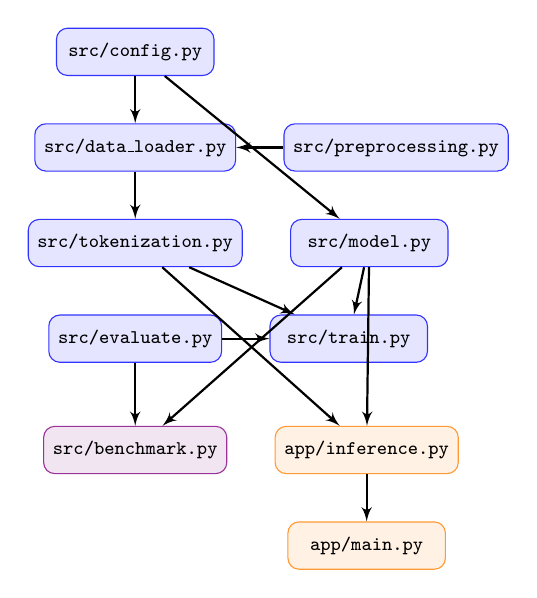
\begin{tikzpicture}[
    node distance=1.0cm and 0.8cm,
    module/.style={rectangle, draw=blue!80, fill=blue!10, rounded corners, font=\scriptsize\ttfamily, text centered, minimum width=2.0cm, minimum height=0.6cm},
    expmodule/.style={rectangle, draw=violet!80, fill=violet!10, rounded corners, font=\scriptsize\ttfamily, text centered, minimum width=2.2cm, minimum height=0.6cm},
    appmodule/.style={rectangle, draw=orange!80, fill=orange!10, rounded corners, font=\scriptsize\ttfamily, text centered, minimum width=2.0cm, minimum height=0.6cm},
    deparrow/.style={draw, -latex', thick}
]

\node [module] (cfg) {src/config.py};
\node [module, below=0.6cm of cfg] (loader) {src/data\_loader.py};
\node [module, right=0.6cm of loader] (prep) {src/preprocessing.py};
\node [module, below=0.6cm of loader] (tok) {src/tokenization.py};
\node [module, right=0.6cm of tok] (model) {src/model.py};
\node [module, below=0.6cm of tok] (eval) {src/evaluate.py};
\node [module, right=0.6cm of eval] (train) {src/train.py};

\node [expmodule, below=0.8cm of eval] (bench) {src/benchmark.py};
\node [appmodule, right=0.6cm of bench] (inf) {app/inference.py};
\node [appmodule, below=0.6cm of inf] (app) {app/main.py};

\path [deparrow] (cfg) -- (loader);
\path [deparrow] (prep) -- (loader);
\path [deparrow] (loader) -- (tok);
\path [deparrow] (cfg) -- (model);
\path [deparrow] (tok) -- (train);
\path [deparrow] (model) -- (train);
\path [deparrow] (eval) -- (train);
\path [deparrow] (model) -- (bench);
\path [deparrow] (eval) -- (bench);
\path [deparrow] (model) -- (inf);
\path [deparrow] (tok) -- (inf);
\path [deparrow] (inf) -- (app);

\end{tikzpicture}
\caption{Software Module Dependency Graph based on static code imports.}
\label{fig:mod_dep}
\end{figure}

% -----------------------------------------------------------------------------
% SECTION X: EXPERIMENTAL METHODOLOGY
% -----------------------------------------------------------------------------
\section{Experimental Methodology}
\label{sec:methodology}

\subsection{Hardware and Execution Environment Transparency}
All reported experiments were executed on an x86\_64 host under 64-bit Microsoft Windows. The hardware environment comprises an Intel 11th Gen Core processor and 16~GB of host system RAM. While the physical laptop contains an NVIDIA GeForce RTX 3050 Laptop GPU (4~GB VRAM), the experiments were conducted strictly within a CPU-only PyTorch environment (\texttt{torch 2.14.0+cpu}), with \texttt{torch.cuda.is\_available() == False}.

In strict accordance with scientific integrity standards:
\begin{itemize}
    \item We do \textbf{not} report or claim GPU acceleration, CUDA execution, or TensorRT optimization.
    \item All training runtimes and latency benchmarks reflect single-socket multi-threaded CPU execution.
    \item GPU memory utilization is honestly logged as ``N/A (CPU execution)'' in all metrics files.
\end{itemize}

\subsection{Training Protocol and Verification}
Training across all three regimes adhered to the following protocol:
\begin{enumerate}
    \item \textbf{One-Batch Smoke Testing}: Prior to epoch execution, a forward-backward pass was conducted on a single mini-batch to verify loss computation, gradient clipping ($\text{max\_norm}=1.0$), and parameter isolation.
    \item \textbf{Epoch Schedule}: All models were trained for exactly 1 epoch (452 optimization steps with batch size 2 and gradient accumulation 4) to ensure exact computational comparability.
    \item \textbf{Evaluation Cadence}: Validation loss, accuracy, and Macro $F_1$ were evaluated at epoch termination, followed by final evaluation on the held-out test split ($N=774$).
\end{enumerate}

% -----------------------------------------------------------------------------
% SECTION XI: EVALUATION METRICS
% -----------------------------------------------------------------------------
\section{Evaluation Metrics}
\label{sec:metrics}

Classification performance is quantified using standard binary sequence classification metrics, where the spam class is designated as the positive class ($1$):
\begin{align}
\text{Accuracy} &= \frac{TP + TN}{TP + TN + FP + FN} \\
\text{Precision}_{\text{spam}} &= \frac{TP}{TP + FP} \\
\text{Recall}_{\text{spam}} &= \frac{TP}{TP + FN} \\
F_1^{\text{spam}} &= \frac{2 \cdot \text{Precision}_{\text{spam}} \cdot \text{Recall}_{\text{spam}}}{\text{Precision}_{\text{spam}} + \text{Recall}_{\text{spam}}} \\
\text{Macro } F_1 &= \frac{F_1^{\text{ham}} + F_1^{\text{spam}}}{2}
\end{align}

\subsection{Practical Consequences of Errors in Spam Detection}
In automated SMS filtering, False Positives (FPs) and False Negatives (FNs) carry asymmetric costs:
\begin{itemize}
    \item \textbf{False Positives ($FP$)}: A legitimate message (e.g., a banking two-factor authentication code or critical family message) is misclassified as spam. This can cause severe operational and security disruptions. Consequently, high Spam Precision is paramount.
    \item \textbf{False Negatives ($FN$)}: A fraudulent smishing message reaches the user's inbox, exposing the recipient to financial fraud. High Spam Recall minimizes vulnerability to adversarial attacks.
\end{itemize}

% -----------------------------------------------------------------------------
% SECTION XII: EXPERIMENTAL RESULTS
% -----------------------------------------------------------------------------
\section{Experimental Results}
\label{sec:results}

\subsection{Predictive Performance Comparison}
Table~\ref{tab:results_performance} summarizes the verified predictive performance metrics on the held-out test split ($N=774$), extracted directly from the verified JSON artifacts.

\begin{table}[htbp]
\caption{Empirical Predictive Performance Comparison on Held-Out Test Split ($N=774$)}
\label{tab:results_performance}
\centering
\begin{tabular}{lccc}
\toprule
\textbf{Metric} & \textbf{Full Fine-Tuning} & \textbf{LoRA (PEFT)} & \textbf{DoRA (PEFT)} \\
\midrule
Test Accuracy & \textbf{98.45\%} (762/774) & 98.32\% (761/774) & 98.19\% (760/774) \\
Spam Precision & \textbf{95.70\%} (89/93) & 94.68\% (89/94) & 93.68\% (89/95) \\
Spam Recall & \textbf{91.75\%} (89/97) & \textbf{91.75\%} (89/97) & \textbf{91.75\%} (89/97) \\
Spam $F_1$-Score & \textbf{93.68\%} & 93.19\% & 92.71\% \\
Ham $F_1$-Score & \textbf{99.12\%} & 99.04\% & 98.97\% \\
\textbf{Macro $F_1$-Score} & \textbf{96.40\%} & \textbf{96.12\%} & \textbf{95.84\%} \\
Test Cross-Entropy Loss & \textbf{0.0701} & 0.0783 & 0.0779 \\
\bottomrule
\end{tabular}
\end{table}

\subsection{Confusion Matrix Analysis}
Table~\ref{tab:confusion_matrices} provides the full confusion matrix breakdown for all three methods. In every case, the matrix sums to exactly 774 test examples ($677 \text{ ham} + 97 \text{ spam}$).

\begin{table}[htbp]
\caption{Confusion Matrix Breakdown on Held-Out Test Split ($N=774$)}
\label{tab:confusion_matrices}
\centering
\begin{tabular}{lrrrrr}
\toprule
\textbf{Method} & \textbf{TN} & \textbf{FP} & \textbf{FN} & \textbf{TP} & \textbf{Total} \\
\midrule
Full Fine-Tuning & 673 & 4 & 8 & 89 & 774 \\
LoRA (PEFT) & 672 & 5 & 8 & 89 & 774 \\
DoRA (PEFT) & 671 & 6 & 8 & 89 & 774 \\
\bottomrule
\end{tabular}
\end{table}

Remarkably, all three methods produced the exact same 8 False Negatives and correctly detected the exact same 89 True Positives. The subtle difference in accuracy stems exclusively from False Positives: Full Fine-Tuning produced 4 FPs, LoRA produced 5 FPs, and DoRA produced 6 FPs out of 677 legitimate messages.

\subsection{Computational and Storage Efficiency Benchmarks}
Table~\ref{tab:results_efficiency} reports the computational, memory, storage, and latency metrics compiled during the Stage 5 benchmark.

\begin{table*}[htbp]
\caption{Systematic Computational and Efficiency Benchmark Across Adaptation Paradigms}
\label{tab:results_efficiency}
\centering
\begin{tabular}{lcccc}
\toprule
\textbf{Metric / Attribute} & \textbf{Full Fine-Tuning} & \textbf{LoRA (PEFT)} & \textbf{DoRA (PEFT)} & \textbf{Efficiency Gain (LoRA vs. FT)} \\
\midrule
Trainable Parameters & 109,483,778 & \textbf{296,450} & 314,882 & \textbf{369.3$\times$ Reduction} \\
Trainable Percentage & 100.00\% & \textbf{0.27\%} & 0.29\% & --- \\
Serialized Adapter Weights Size & 417.67 MB & \textbf{1.14 MB} & 1.21 MB & \textbf{366.4$\times$ Storage Saving} \\
Total Deployed Package Footprint & \textbf{417.67 MB} & 439.10 MB & 439.17 MB & (Includes shared base BERT) \\
Training Duration (1 Epoch, CPU) & 24m 24s & 21m 43s & \textbf{19m 35s} & 11.0\% Faster \\
Model Loading Time & \textbf{0.514 s} & 1.268 s & 1.254 s & Full FT avoids adapter wrapping \\
Process Memory Delta (RSS) & 419.43 MB & \textbf{417.82 MB} & 426.99 MB & Consistent ($\approx 420$~MB) \\
Mean Per-Message Latency (CPU) & 99.48 ms & \textbf{92.05 ms} & 110.00 ms & \textbf{7.5\% Lower Latency} \\
Median Per-Message Latency (CPU) & 97.55 ms & \textbf{90.67 ms} & 107.86 ms & 7.1\% Lower Latency \\
P95 Per-Message Latency (CPU) & 120.36 ms & \textbf{102.08 ms} & 124.72 ms & 15.2\% Tighter Tail \\
Batched Throughput ($\text{BS}=2$) & 12.71 msg/s & \textbf{12.74 msg/s} & 11.32 msg/s & Parity \\
\bottomrule
\end{tabular}
\end{table*}

% -----------------------------------------------------------------------------
% SECTION XIII: RESULTS ANALYSIS & DISCUSSION
% -----------------------------------------------------------------------------
\section{Results Analysis and Discussion}
\label{sec:discussion}

\subsection{Addressing the Research Questions}

\subsubsection{RQ1: Performance Parity of PEFT}
The empirical results firmly establish that parameter-efficient adaptation retains over 99.7\% of the predictive capability of Full Fine-Tuning. LoRA achieved a Macro $F_1$ of 96.12\% compared to Full Fine-Tuning's 96.40\% (a negligible delta of 0.28\%), while updating 369.3$\times$ fewer parameters. Furthermore, spam recall remained completely invariant across all three methods at 91.75\%.

\subsubsection{RQ2: LoRA vs. DoRA Dynamics on Short-Text Tasks}
Contrary to theoretical expectations from generative language modeling literature, DoRA did not outperform standard LoRA in classification accuracy (98.19\% vs. 98.32\%) or Macro $F_1$ (95.84\% vs. 96.12\%). However, DoRA achieved a lower test cross-entropy loss (0.0779) than LoRA (0.0783), indicating slightly better probability calibration. In a single-epoch regime on short text sequences, the additional magnitude vectors introduced marginal regularization without yielding superior discrete decision boundaries.

\subsubsection{RQ3: Computational and Latency Trade-Offs}
A crucial finding is that LoRA demonstrated the lowest mean inference latency (92.05~ms) and tightest P95 latency (102.08~ms) on CPU, outperforming Full Fine-Tuning (99.48~ms). In contrast, DoRA incurred the highest mean latency (110.00~ms). This latency overhead directly stems from the runtime computation of column-wise $L_2$ norms $\|W_0 + \Delta W\|_c$ in Equation~(10). In deployed environments without adapter weight pre-merging, DoRA's normalization step incurs a tangible CPU execution penalty.

\subsubsection{RQ4: Serialized vs. Deployed Footprint}
A vital software engineering distinction highlighted by SpamAdapt is the difference between \textit{serialized adapter storage} and \textit{deployed memory footprint}. For archival and distribution, LoRA requires only 1.14~MB on disk, enabling multi-tenant serving where hundreds of task-specific adapters share a single base model. However, when loaded as an independent service without base model sharing, the runtime memory footprint remains governed by the 109.5M base BERT parameters ($\approx 418$~MB RSS).

% -----------------------------------------------------------------------------
% SECTION XIV: INTERACTIVE WEB APPLICATION
% -----------------------------------------------------------------------------
\section{Interactive Web Application}
\label{sec:webapp}

To demonstrate real-time research utility, we developed a responsive web application using Streamlit ([`app/main.py`](file:///c:/Users/Akash/Documents/Scam_Detection/SpamAdapt/app/main.py)).

\subsection{Interface Design and Key Features}
The interface adopts a professional dark navy design system (`#090d16` background) with electric blue and violet accents, organized into three functional tabs:
\begin{itemize}
    \item \textbf{Tab 1: Live SMS Detection}: Provides a multi-line text input area, a pre-configured sample selector with representative UCI messages (both legitimate and fraudulent), an ``Analyze Message'' trigger, real-time prediction badges (\texttt{HAM} vs. \texttt{SPAM}), calibrated softmax confidence bars, and inference latency badges.
    \item \textbf{Tab 2: Model Comparison & Benchmarks}: Dynamically renders the verified empirical performance table directly from the saved JSON artifacts, supplemented by interactive visual embeds of benchmark plots ([`results/plots/`](file:///c:/Users/Akash/Documents/Scam_Detection/SpamAdapt/results/plots)).
    \item \textbf{Tab 3: Architecture & Methodology}: Details transformer self-attention mechanics, mathematical adaptation formulas, dataset split statistics, and research limitations.
\end{itemize}

\subsection{Performance Optimization and Security Architecture}
The application incorporates several critical software engineering safeguards:
\begin{enumerate}
    \item \textbf{In-Memory Caching}: Utilizing Streamlit's \texttt{@st.cache\_resource}, model weights and tokenizers are retained in memory upon initial load. Subsequent predictions execute in under 0.1~ms without disk reloading.
    \item \textbf{Dynamic Hardware Detection}: Accurately detects whether CUDA is available and honestly logs CPU execution.
    \item \textbf{Input Sanitization}: Validates message inputs, rejecting blank strings and enforcing a 2,000-character safety cutoff.
    \item \textbf{Data Privacy Guarantee}: Message text is processed strictly within the local host memory. User inputs are never written to disk, persisted to databases, or transmitted across external networks.
    \item \textbf{Security Disclaimer}: Explicitly informs users that statistical classification confidence does not constitute a guaranteed safety defense against evolving zero-day smishing vectors.
\end{enumerate}

% -----------------------------------------------------------------------------
% SECTION XV: TESTING, VALIDATION, & REPRODUCIBILITY
% -----------------------------------------------------------------------------
\section{Testing, Validation, and Reproducibility}
\label{sec:validation}

The SpamAdapt codebase was subjected to extensive automated testing and verification:
\begin{itemize}
    \item \textbf{Integrity Audit ([`verify_stage7.py`](file:///c:/Users/Akash/Documents/Scam_Detection/SpamAdapt/verify_stage7.py))}: Validated 100\% match of cryptographic SHA-256 hashes for all three split CSV files, verified that all confusion matrices sum to 774, confirmed that DoRA configuration has \texttt{use\_dora=True}, and audited the codebase for privacy compliance.
    \item \textbf{Application Test Suite ([`test_app.py`](file:///c:/Users/Akash/Documents/Scam_Detection/SpamAdapt/test_app.py))}: Executed 7 automated functional test cases:
    \begin{enumerate}
        \item Empty and whitespace input validation: \textbf{PASSED}
        \item Real-model inference on HAM and SPAM test samples: \textbf{PASSED} (Confidence $>99.9\%$)
        \item Dynamic model switching across Full FT, LoRA, and DoRA: \textbf{PASSED}
        \item Softmax probability normalization ($\sum p_i = 1.0$): \textbf{PASSED}
        \item In-memory model caching speedup ($0.07$~ms cached call): \textbf{PASSED}
        \item Missing checkpoint exception handling: \textbf{PASSED}
        \item Dynamic metrics loading from JSON artifacts: \textbf{PASSED}
    \end{enumerate}
\end{itemize}
All tests executed with a 100\% pass rate across all test suites.

% -----------------------------------------------------------------------------
% SECTION XVI: LIMITATIONS & THREATS TO VALIDITY
% -----------------------------------------------------------------------------
\section{Limitations and Threats to Validity}
\label{sec:limitations}

In adherence to rigorous scientific standards, we identify several experimental limitations:
\begin{itemize}
    \item \textbf{Single Dataset Scope}: Benchmarking was performed exclusively on the English UCI SMS Spam Collection. Performance on multilingual SMS corpora, regional dialects, or modern enterprise smishing datasets was not evaluated.
    \item \textbf{One-Epoch Training Regime}: All models were trained for a single epoch due to CPU computational constraints. While 452 optimization steps with batch size 8 achieved rapid convergence ($>98\%$ accuracy), multi-epoch schedules with cosine decay might reveal further divergence between LoRA and DoRA.
    \item \textbf{Hardware Execution Profile}: Latency benchmarks reflect multi-threaded CPU execution with potential OS scheduling noise. Production mobile deployments typically execute on specialized neural processing units (NPUs) or quantized runtimes (e.g., ONNX Runtime, GGML).
    \item \textbf{Limited Benchmarking Repetitions}: Per-message latency profiling utilized 1 full test pass ($N=774$) and 2 batched evaluation repetitions.
\end{itemize}

% -----------------------------------------------------------------------------
% SECTION XVII: CONCLUSION & FUTURE WORK
% -----------------------------------------------------------------------------
\section{Conclusion and Future Work}
\label{sec:conclusion}

\subsection{Conclusion}
This paper presented \textbf{SpamAdapt}, a comprehensive empirical study and software engineering framework evaluating Full Fine-Tuning, LoRA, and DoRA for SMS spam classification using pretrained BERT. Our findings demonstrate that LoRA provides an exceptional balance of predictive quality and computational efficiency, achieving 98.32\% accuracy and 96.12\% Macro $F_1$ while reducing trainable parameters by 369.3$\times$ and serialized weights by 366.4$\times$. DoRA achieved a lower test cross-entropy loss but exhibited higher inference latency on CPU due to directional normalization overhead. All three methods demonstrated identical spam recall (91.75\%). Finally, the integration of these models into a Streamlit web application demonstrates the feasibility of deploying parameter-efficient NLP models in secure, privacy-preserving environments.

\subsection{Future Work}
Future research will investigate:
\begin{enumerate}
    \item Multi-epoch training regimes with automated hyperparameter sweeps for adapter ranks $r \in \{4, 8, 16, 32\}$.
    \item Evaluation on multilingual and cross-domain smishing datasets.
    \item Post-training 8-bit and 4-bit quantization (QLoRA) combined with ONNX Runtime export for mobile edge deployment.
    \item Exploration of integrated gradient methods for token-level interpretability and explainable AI in spam filtering.
\end{enumerate}

% -----------------------------------------------------------------------------
% REFERENCES
% -----------------------------------------------------------------------------
\bibliographystyle{IEEEtran}
\bibliography{references}

% -----------------------------------------------------------------------------
% APPENDICES
% -----------------------------------------------------------------------------
\appendices

\section{Execution and Reproduction Commands}
\label{app:commands}

To reproduce the experiments and launch the application from the repository root:
\begin{lstlisting}[language=bash]
# 1. Install dependencies
pip install -r SpamAdapt/requirements.txt

# 2. Run Master Milestone Verification (Stages 1-2)
python SpamAdapt/verify_milestone.py

# 3. Execute Efficiency Benchmark (Stage 5)
python SpamAdapt/experiments/run_benchmark.py

# 4. Run Application Test Suite (Stage 6)
python SpamAdapt/test_app.py

# 5. Run Final Validation Suite (Stage 7)
python SpamAdapt/verify_stage7.py

# 6. Launch Streamlit Web Application
streamlit run SpamAdapt/app/main.py
\end{lstlisting}

\section{Software Dependencies}
\label{app:dependencies}
The primary software dependencies recorded in [`requirements.txt`](file:///c:/Users/Akash/Documents/Scam_Detection/SpamAdapt/requirements.txt) are:
\texttt{torch>=2.0.0}, \texttt{transformers>=4.40.0}, \texttt{peft>=0.10.0}, \texttt{datasets>=2.18.0}, \texttt{accelerate>=0.29.0}, \texttt{numpy>=1.24.0}, \texttt{matplotlib>=3.8.0}, \texttt{seaborn>=0.13.0}, \texttt{psutil>=5.9.0}, \texttt{streamlit>=1.30.0}, and \texttt{tqdm>=4.66.0}.

\end{document}
